\documentclass[track=junior,level=1]{kidscode}
%% a picture to circle: \pick{icon}{word}
\newcommand{\pick}[2]{\begin{tabular}{@{}c@{}}{\fontsize{34}{40}\selectfont #1}\\[4pt]\textbf{#2}\end{tabular}}
%% a row of faces to circle for the child self-rating
\newcommand{\faces}{{\LARGE\faFrown[regular]\quad\faMeh[regular]\quad\faSmile[regular]}}
\newenvironment{howami}{\par\noindent\renewcommand{\arraystretch}{1.6}%
  \tabularx{\linewidth}{@{}>{\RaggedRight}X>{\centering\arraybackslash}p{4.6cm}@{}}
  \toprule \rowcolor{kcaccent!15}\textbf{Read it aloud} & \textbf{Circle a face}\\ \midrule}
  {\bottomrule\endtabularx\par}
\newcommand{\howrow}[1]{#1 & \faces\\}
\begin{document}
\kctitle{Show-Me Checklists}{Week 1 chat, week 5 and week 10 show-me checklists. One copy per child}

\begin{grownup}[These are not tests]
Nothing here is a test or a grade. You watch your child play and build, and check off what you
see. Print one copy of each page per child, in the week you use it. If a row did not come up
naturally, ask \enquote{Can you show me how you\dots?} at the end of the session. The Answer Key
(\enquote{How to use the show-me checklists}) says what each column looks like and what to do next.
\end{grownup}

\begin{center}\renewcommand{\arraystretch}{1.4}
\begin{tabularx}{\linewidth}{@{}>{\bfseries}p{3.4cm}X@{}}
\toprule
Not yet & Needs you to show it, or does not try it yet. That is fine: it is new.\\
Getting there & Does it with a hint, a reminder or a look at the book.\\
Got it & Does it alone, and can show it again another day.\\
\bottomrule
\end{tabularx}
\end{center}

%% =====================================================================
\kcpart{Week 1}{What Do You Like to Make?}{A 5-minute chat. Not graded. There are no wrong answers.}

Nickname: \rule{6cm}{0.4pt}\hfill Date: \rule{3.5cm}{0.4pt}

\begin{grownup}[How to run the chat]
Sit side by side, read each question aloud and let your child circle (or point while you circle).
Keep it light and short. Write anything they say in the notes box.
\end{grownup}

\section{1. What do you like? Circle all you like.}
\begin{center}
%% alt: Five pictures to circle in a row: a paw for animals, a game controller for games, an open book for stories, a music note for music and a paintbrush for drawing.
\begin{tikzpicture}
  \foreach \icon/\word [count=\i] in {\faPaw/animals,\faGamepad/games,\faBookOpen/stories,\faMusic/music,\faPaintBrush/drawing}
    \node[align=center] at (\i*3.3,0) {\pick{\icon}{\word}};
\end{tikzpicture}
\end{center}
Something else you love to make or do (say it or draw it):
\answerspace{3cm}

\section{2. How do you feel about computers? Circle one.}
\begin{center}
\renewcommand{\arraystretch}{1.6}
\begin{tabular}{cccc}
{\fontsize{34}{40}\selectfont\faFrown[regular]} & {\fontsize{34}{40}\selectfont\faMeh[regular]} & {\fontsize{34}{40}\selectfont\faSmile[regular]} & {\fontsize{34}{40}\selectfont\faGrinStars[regular]}\\
worried & not sure & happy & super excited\\
\end{tabular}
\end{center}

\section{3. What would you like to make on the computer?}
Draw it here.
\answerspace{5cm}

\begin{grownup}[Questions you can ask]
\enquote{Have you used a computer or a tablet before? What did you do on it?}
\enquote{Do you like to go first, or watch first?}
\enquote{What would you like to make a cat do?}
\end{grownup}

\textbf{Notes for next time} (for the grown-up):
\answerspace{3.5cm}

%% =====================================================================
\kcpart{Week 5}{Show Me: Play Day}{Watch during the play day. Check one box in each row.}

Nickname: \rule{6cm}{0.4pt}\hfill Date: \rule{3.5cm}{0.4pt}
\medskip

\begin{showme}[Week 5]
\showmerow{put arrow cards in order to reach a goal}
\showmerow{snap a green-flag script together}
\showmerow{use repeat to do something again}
\showmerow{find and fix a block that is not snapped on or is in the wrong order}
\showmerow{take turns as Driver and Helper}
\showmerow{say what their script does}
\end{showme}

\medskip
\textbf{Notes for next time} (what to practice, what to celebrate):
\answerspace{4cm}

\section{How am I doing?}
\begin{grownup}
Read each line aloud. Your child circles a face. Every face is a good answer.
\end{grownup}
\begin{howami}
\howrow{I can give a robot steps in order.}
\howrow{I can make the cat move with the green flag.}
\howrow{I can use repeat.}
\howrow{I can fix a bug.}
\howrow{I can share the mouse.}
\end{howami}

%% =====================================================================
\kcpart{Week 10}{Show Me: Showcase}{Watch during project time and the showcase. Check one box in each row.}

Nickname: \rule{6cm}{0.4pt}\hfill Date: \rule{3.5cm}{0.4pt}
\medskip

\begin{showme}[Week 10]
\showmerow{start a script with the green flag, a click or a key}
\showmerow{use repeat for an animation or a dance}
\showmerow{use two sprites or a backdrop change}
\showmerow{draw a shape with the pen}
\showmerow{plan with a storyboard and build it}
\showmerow{find and fix a bug}
\showmerow{explain one script}
\showmerow{use nicknames and give credit}
\end{showme}

\medskip
\textbf{Notes for next time} (to pass on to Junior Level 2):
\answerspace{4cm}

\section{How am I doing?}
\begin{grownup}
Read each line aloud. Your child circles a face. Look back at week 5 together: what can you do now?
\end{grownup}
\begin{howami}
\howrow{I can start my card with a click or a key.}
\howrow{I can make a sprite dance with repeat.}
\howrow{I can draw a square with the pen.}
\howrow{I can plan on a storyboard.}
\howrow{I can fix a bug.}
\howrow{I can tell someone what my script does.}
\end{howami}

\end{document}
